\documentclass[notes,11pt, aspectratio=169]{beamer}

\usepackage{pgfpages}
% These slides also contain speaker notes. You can print just the slides,
% just the notes, or both, depending on the setting below. Comment out the want
% you want.
\setbeameroption{hide notes} % Only slide
%\setbeameroption{show only notes} % Only notes
%\setbeameroption{show notes on second screen=right} % Both

%\usepackage[scaled=1.0]{helvet}
\usepackage{array}


\usepackage{tikz}
\usetikzlibrary{calc}
\usetikzlibrary{matrix}
\usetikzlibrary{positioning}


\usepackage{verbatim}
\setbeamertemplate{note page}{\pagecolor{gray!5}\insertnote}
\usetikzlibrary{positioning}
\usetikzlibrary{snakes}
\usetikzlibrary{calc}
\usetikzlibrary{arrows}
\usetikzlibrary{decorations.markings}
\usetikzlibrary{shapes.misc}
\usetikzlibrary{matrix,shapes,arrows,fit,tikzmark}
\usepackage{amsmath}
\usepackage{mathpazo}
\usepackage{hyperref}
\usepackage{lipsum}
\usepackage{multimedia}
\usepackage{graphicx}
\usepackage{multirow}
\usepackage{graphicx}
\usepackage{dcolumn}
\usepackage{bbm}
\newcolumntype{d}[0]{D{.}{.}{5}}

\usepackage{changepage}
\usepackage{appendixnumberbeamer}
\newcommand{\beginbackup}{
   \newcounter{framenumbervorappendix}
   \setcounter{framenumbervorappendix}{\value{framenumber}}
   \setbeamertemplate{footline}
   {
     \leavevmode%
     \hline
     box{%
       \begin{beamercolorbox}[wd=\paperwidth,ht=2.25ex,dp=1ex,right]{footlinecolor}%
%         \insertframenumber  \hspace*{2ex} 
       \end{beamercolorbox}}%
     \vskip0pt%
   }
 }
\newcommand{\backupend}{
   \addtocounter{framenumbervorappendix}{-\value{framenumber}}
   \addtocounter{framenumber}{\value{framenumbervorappendix}} 
}


\usepackage{graphicx}
\usepackage[space]{grffile}
\usepackage{booktabs}

% These are my colors -- there are many like them, but these ones are mine.
\definecolor{blue}{RGB}{0,114,178}
\definecolor{red}{RGB}{213,94,0}
\definecolor{yellow}{RGB}{240,228,66}
\definecolor{green}{RGB}{0,158,115}

\hypersetup{
  colorlinks=false,
  linkbordercolor = {white},
  linkcolor = {blue}
}

\usepackage{graphicx,stackengine,xcolor}
\newcommand\Circle[1]{%
	\def\useanchorwidth{T}%
	\def\stacktype{L}%
	\stackon[0pt]{#1}{\scalebox{2.0}[1.15]{\textcolor{red}{$\bigcirc$}}}%
}

%% I use a beige off white for my background
\definecolor{MyBackground}{RGB}{255,253,218}

%% Uncomment this if you want to change the background color to something else
%\setbeamercolor{background canvas}{bg=MyBackground}

%% Change the bg color to adjust your transition slide background color!
\newenvironment{transitionframe}{
  \setbeamercolor{background canvas}{bg=white}
  \begin{frame}}{
    \end{frame}
}

\setbeamercolor{frametitle}{fg=blue}
\setbeamercolor{title}{fg=black}
\setbeamertemplate{footline}[frame number]
\setbeamertemplate{navigation symbols}{} 
\setbeamertemplate{itemize items}{-}
\setbeamercolor{itemize item}{fg=blue}
\setbeamercolor{itemize subitem}{fg=blue}
\setbeamercolor{enumerate item}{fg=blue}
\setbeamercolor{enumerate subitem}{fg=blue}
\setbeamercolor{button}{bg=MyBackground,fg=blue,}

%%% TIKZ STUFF
\tikzset{   
	every picture/.style={remember picture,baseline},
	every node/.style={anchor=base,align=center,outer sep=1.5pt},
	every path/.style={thick},
}
\newcommand\marktopleft[1]{%
	\tikz[overlay,remember picture] 
	\node (marker-#1-a) at (-.3em,.3em) {};%
}
\newcommand\markbottomright[2]{%
	\tikz[overlay,remember picture] 
	\node (marker-#1-b) at (0em,0em) {};%
}
\tikzstyle{every picture}+=[remember picture] 
\tikzstyle{mybox} =[draw=black, very thick, rectangle, inner sep=10pt, inner ysep=20pt]
\tikzstyle{fancytitle} =[draw=black,fill=red, text=white]
%%%% END TIKZ STUFF


% If you like road maps, rather than having clutter at the top, have a roadmap show up at the end of each section 
% (and after your introduction)
% Uncomment this is if you want the roadmap!
% \AtBeginSection[]
% {
%    \begin{frame}
%        \frametitle{Roadmap of Talk}
%        \tableofcontents[currentsection]
%    \end{frame}
% }
\setbeamercolor{section in toc}{fg=blue}
\setbeamercolor{subsection in toc}{fg=red}
\setbeamersize{text margin left=1em,text margin right=1em} 

\newenvironment{wideitemize}{\itemize\addtolength{\itemsep}{10pt}}{\enditemize}
\newenvironment{wideenumerate}{\enumerate\addtolength{\itemsep}{10pt}}{\endenumerate}

\usepackage{environ}
\NewEnviron{videoframe}[1]{
  \begin{frame}
    \vspace{-8pt}
    \begin{columns}[onlytextwidth, T] % align columns
      \begin{column}{.58\textwidth}
        \begin{minipage}[t][\textheight][t]
          {\dimexpr\textwidth}
          \vspace{8pt}
          \hspace{4pt} {\Large \sc \textcolor{blue}{#1}}
          \vspace{8pt}
          
          \BODY
        \end{minipage}
      \end{column}%
      \hfill%
      \begin{column}{.42\textwidth}
        \colorbox{green!20}{\begin{minipage}[t][1.2\textheight][t]
            {\dimexpr\textwidth}
            Face goes here
          \end{minipage}}
      \end{column}%
    \end{columns}
  \end{frame}
}

\title[]{\textcolor{blue}{ECN 453: Game Theory 1}}
\author[PGP]{}
\institute[FRBNY]{\small{\begin{tabular}{c c c}
Nicholas Vreugdenhil \\
\end{tabular}}}
\date{} 

\begin{document}

% Title Slide
\begin{frame}
\maketitle
  \centering
\end{frame}

% INTRO

\begin{frame}{Strategic decision making}
\begin{wideitemize}
	\item So far, we have seen models of \textit{independent} decision making.
	\item In other words, when firms made their optimal choices (for example, choosing optimal prices) they did not need to think about what other firms were doing.
	\begin{wideitemize}
		\item For example, in monopoly, there were no other firms in the market!
	\end{wideitemize} 
	\item Today, we will study \textbf{game theory}. 
	\item These are models where optimal choices are \textit{strategic}: a firm's optimal choice depends on what other firms are doing.
	\item Much of what we will see in this lecture is review from previous courses. We will build on this review in future lectures.
\end{wideitemize}
\end{frame}

\begin{frame}{Example of strategic decision making}
	\begin{wideitemize}
		\item Two hollywood studios in 2010: Warner Bros and Fox, deciding when to release their blockbuster movies: Harry Potter, Chronicles of Narnia.
	\end{wideitemize}
	\begin{figure}
		\includegraphics[scale=0.1]{harry_potter.jpeg}
		\hspace{50pt}
		\includegraphics[scale=0.2]{narnia.jpeg}
	\end{figure}
\end{frame}

\begin{frame}{Example of strategic decision making (continued)}
	\begin{wideitemize}
		\item Which month should the studios release their movie: December or November?
		\item Consider the decision of Warner Bros who are thinking about when to release the Harry Potter movie. \pause
		\begin{wideitemize}
				\vspace{11pt}
				\item December is in the holidays so it's a better month to release Harry Potter if it is the only movie because it will get a bigger audience.
				\item But: if Fox decides to release Narnia in December, the audience for the Harry Potter movie will be split.
				\item So, if Fox decides to release Narnia in December, it will be better to release the Harry Potter movie in November.
			\end{wideitemize}
		\item So: the decision of one movie studio about when to release the movie depends on the choices of the \textit{other} movie studio. It is \textit{strategic}.
		\begin{wideitemize}
			\vspace{11pt}
			\item  Game theory can be used to model and understand strategic decisions like these.
		\end{wideitemize}
	\end{wideitemize}
\end{frame}

\begin{frame}{Plan}
	  \begin{wideenumerate}
		\item \textbf{Simultaneous games: setup and Nash equilibrium}
		\item Simultaneous games: dominant and dominated strategies
	\end{wideenumerate}
\end{frame}

\begin{frame}{Simultaneous games: setup}
	\begin{wideitemize}
		  	\item We will start by studying \textbf{simultaneous games}.
		  	\item These are games where choices are made at the same time.
		  	\begin{wideitemize}
		  		\vspace{11pt}
		  		\item By contrast, we will next study \textit{sequential games} where firms makes choices one after the other.
		  	\end{wideitemize}
	  		\item I will begin by defining some important language that economists use when talking about game theory.
	\end{wideitemize}
\end{frame}

\begin{frame}{Simultaneous games: setup}{It's very important that you can identify the following components from the figure on the right.}

\begin{columns}[onlytextwidth, T]
		\begin{column}{.45\textwidth}
		\vspace{20pt}
		\hspace{20pt}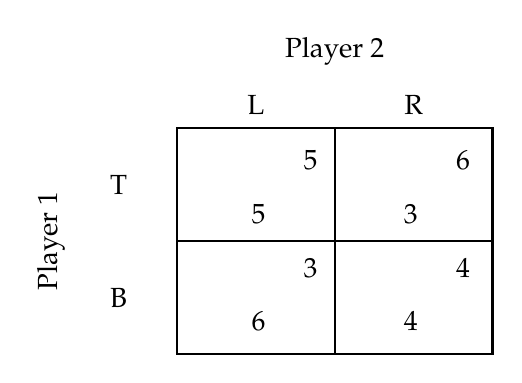
\begin{tikzpicture}
			\matrix[matrix of math nodes,
			every odd row/.style={align=right},every evenrow/.style={align=left},every node/.style={text width=1.5cm},row sep=0.2cm,column sep=0.2cm,ampersand replacement=\&] (m) {
				5\&6 \\
				5\&3 \\
				3 \&4 \\
				6 \&4\\
			};
			\draw (m.north east) rectangle (m.south west);
			\draw (m.north) -- (m.south);
			\draw (m.east) -- (m.west);
			
			% Player 1
			\coordinate (c) at ($(m.north west)!0.25!(m.south west)$);
			\coordinate (d) at ($(m.north west)!0.75!(m.south west)$);
			\node[left=2pt of c,text width=1cm]  {T};
			\node[left=2pt of d,text width=1cm]  {B};
			
			% Player 2
			\coordinate (a) at ($(m.north west)!0.25!(m.north east)$);
			\coordinate (b) at ($(m.north west)!0.75!(m.north east)$);
			\node[above=5pt of a,anchor=base] {L};
			\node[above=5pt of b,anchor=base] {R};
			
			\node[above=18pt of m.north] (firm b) {Player 2};
			\node[left=1.6cm of m.west,rotate=90,align=center,anchor=center] {Player 1};
			
			%\node[above=5pt of firm b]  {Payoff Matrix};
		\end{tikzpicture}
	\end{column} 
	\begin{column}{.55\textwidth}
	\begin{wideitemize}
		\item \textbf{Players}: \pause Player 1 and Player 2
		\item \textbf{Strategies} \pause
			\begin{wideitemize}
				\item Player 1 has strategies `T' and `B'
				\item Player 2 has strategies `L' and `R'
			\end{wideitemize}
		\item \textbf{Payoffs}: \pause the numbers in the matrix
			\begin{wideitemize}
				\item Higher payoffs are better
				\item Payoffs depend on the choices of \textit{both players}
				\item E.g. if Player 1 chooses `T', Player 2 chooses `R' then:
				\begin{wideitemize}
				 	\item Player 1 receives payoff = 3
				 	\item Player 2 receives payoff = 6. 
				 \end{wideitemize}
			\end{wideitemize}
	\end{wideitemize}
	\end{column}

	\end{columns}
\end{frame}

\begin{frame}{Simultaneous games: setup}
\begin{columns}[onlytextwidth, T] 
		\begin{column}{.45\textwidth}
		\vspace{20pt}
		\hspace{20pt}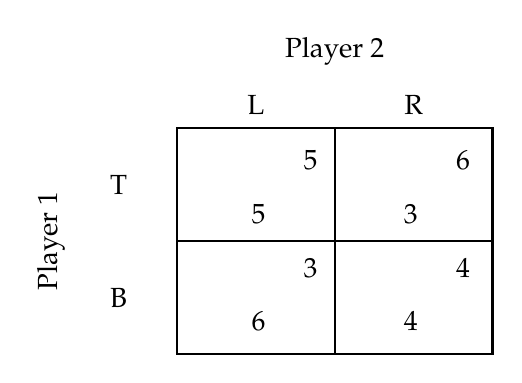
\begin{tikzpicture}
			\matrix[matrix of math nodes,
			every odd row/.style={align=right},every evenrow/.style={align=left},every node/.style={text width=1.5cm},row sep=0.2cm,column sep=0.2cm,ampersand replacement=\&] (m) {
				5\&6 \\
				5\&3 \\
				3 \&4 \\
				6 \&4\\
			};
			\draw (m.north east) rectangle (m.south west);
			\draw (m.north) -- (m.south);
			\draw (m.east) -- (m.west);
			
			% Player 1
			\coordinate (c) at ($(m.north west)!0.25!(m.south west)$);
			\coordinate (d) at ($(m.north west)!0.75!(m.south west)$);
			\node[left=2pt of c,text width=1cm]  {T};
			\node[left=2pt of d,text width=1cm]  {B};
			
			% Player 2
			\coordinate (a) at ($(m.north west)!0.25!(m.north east)$);
			\coordinate (b) at ($(m.north west)!0.75!(m.north east)$);
			\node[above=5pt of a,anchor=base] {L};
			\node[above=5pt of b,anchor=base] {R};
			
			\node[above=18pt of m.north] (firm b) {Player 2};
			\node[left=1.6cm of m.west,rotate=90,align=center,anchor=center] {Player 1};
			
			%\node[above=5pt of firm b]  {Payoff Matrix};
		\end{tikzpicture}
	\end{column}
	\begin{column}{.55\textwidth}
		\begin{wideitemize}
			\item Representing the elements (players, strategies, payoffs) in this form is called the `normal form' of a game.
		\end{wideitemize}
	\end{column}
\end{columns}
\end{frame}

\begin{frame}{Simultaneous games: best responses}
	
	\begin{columns}[onlytextwidth, T] 
		
		\begin{column}{.45\textwidth}
			\vspace{30pt}
			\hspace{20pt} 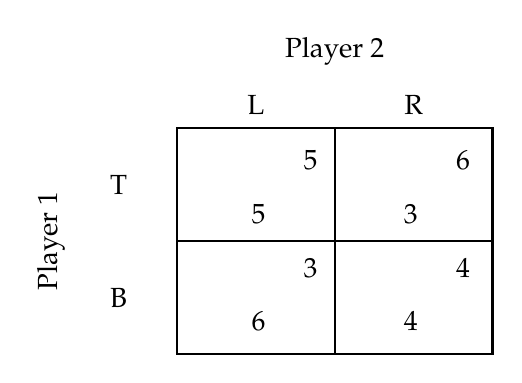
\begin{tikzpicture}
				\matrix[matrix of math nodes,every odd row/.style={align=right},every evenrow/.style={align=left},every node/.style={text width=1.5cm},row sep=0.2cm,column sep=0.2cm,ampersand replacement=\&] (m) {
					5\&6 \\
					5\&3 \\
					3 \&4 \\
					6 \&4\\
				};
				\draw (m.north east) rectangle (m.south west);
				\draw (m.north) -- (m.south);
				\draw (m.east) -- (m.west);
				
				% Player 1
				\coordinate (c) at ($(m.north west)!0.25!(m.south west)$);
				\coordinate (d) at ($(m.north west)!0.75!(m.south west)$);
				\node[left=2pt of c,text width=1cm]  {T};
				\node[left=2pt of d,text width=1cm]  {B};
				
				% Player 2
				\coordinate (a) at ($(m.north west)!0.25!(m.north east)$);
				\coordinate (b) at ($(m.north west)!0.75!(m.north east)$);
				\node[above=5pt of a,anchor=base] {L};
				\node[above=5pt of b,anchor=base] {R};
				
				\node[above=18pt of m.north] (firm b) {Player 2};
				\node[left=1.6cm of m.west,rotate=90,align=center,anchor=center] {Player 1};
				
				%\node[above=5pt of firm b]  {Payoff Matrix};
			\end{tikzpicture}
		\end{column}
		\begin{column}{.55\textwidth}
			\begin{wideitemize}
				\item \textbf{Best response}: \pause the optimal strategy for a player \textit{given} the choice of the other player.
				\item Notation: ``best response of player 1 given that player 2 chooses R'' written as:
				\begin{align*}
					BR_1(R)
				\end{align*}
				\item We can find the best response by finding the strategy with the highest payoff given a choice by the other player.
				\item \textbf{Example:} $BR_1(R)=B$. 
				\item Why? Given player 2 plays R, player 1 gets:
				\begin{wideitemize}
				 \item Payoff=3 if play T $<$ payoff=4 if play B.
				 \end{wideitemize}
			\end{wideitemize}
		\end{column}
	\end{columns}
\end{frame}



\begin{frame}{Simultaneous games: best responses}
	
	\begin{columns}[onlytextwidth, T] 
				\begin{column}{.45\textwidth}
			%\vspace{30pt}
			\hspace{20pt} 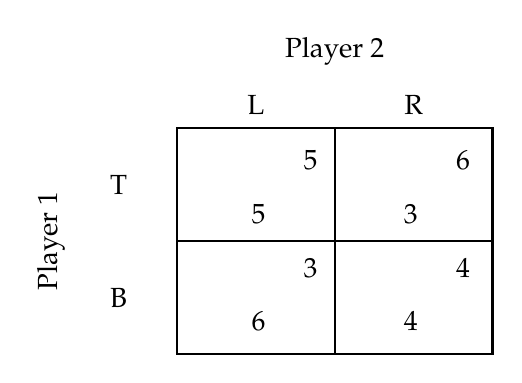
\begin{tikzpicture}
				\matrix[matrix of math nodes,every odd row/.style={align=right},every evenrow/.style={align=left},every node/.style={text width=1.5cm},row sep=0.2cm,column sep=0.2cm,ampersand replacement=\&] (m) {
					5\&6 \\
					5\&3 \\
					3 \&4 \\
					6 \&4\\
				};
				\draw (m.north east) rectangle (m.south west);
				\draw (m.north) -- (m.south);
				\draw (m.east) -- (m.west);
				
				% Player 1
				\coordinate (c) at ($(m.north west)!0.25!(m.south west)$);
				\coordinate (d) at ($(m.north west)!0.75!(m.south west)$);
				\node[left=2pt of c,text width=1cm]  {T};
				\node[left=2pt of d,text width=1cm]  {B};
				
				% Player 2
				\coordinate (a) at ($(m.north west)!0.25!(m.north east)$);
				\coordinate (b) at ($(m.north west)!0.75!(m.north east)$);
				\node[above=5pt of a,anchor=base] {L};
				\node[above=5pt of b,anchor=base] {R};
				
				\node[above=18pt of m.north] (firm b) {Player 2};
				\node[left=1.6cm of m.west,rotate=90,align=center,anchor=center] {Player 1};
				
				%\node[above=5pt of firm b]  {Payoff Matrix};
			\end{tikzpicture}
		\end{column}
		\begin{column}{.55\textwidth}
			\begin{wideitemize}
				\item Let's find some more best responses.
				\item $BR_1(L) = B$
				\begin{wideitemize}
					\item Payoff=5 if play T $<$ payoff=6 if play B.
				\end{wideitemize}
				\item $BR_2(T) = R$
				\begin{wideitemize}
					\item Payoff=5 if play L $<$ payoff=6 if play R.
				\end{wideitemize}
				\item $BR_2(B) = R$
				\begin{wideitemize}
					\item Payoff=3 if play L $<$ payoff=4 if play R.
				\end{wideitemize}
			\end{wideitemize}
		\end{column}
	\end{columns}
\end{frame}

\begin{frame}{Simultaneous games: Nash equilibrium}
	\begin{wideitemize}
		\item Where do we expect the game to end up? A \textbf{Nash equilibrium}: \pause
		\begin{center}
			\vspace{11pt}
			\textit{A pair of strategies constitutes a Nash equilibrium if no player can unilaterally change its strategy in a way that improves its payoff.}
		\end{center}
		\item So, a Nash equilibrium occurs when each player is choosing a best response to the other player's choice.
		\end{wideitemize}
\end{frame}

\begin{frame}{Simultaneous games: Nash equilibrium}
	\begin{wideitemize}
		\item In practice we can find a Nash equilibrium using the following steps:
	\end{wideitemize}
	\begin{enumerate}
		\vspace{11pt}
		\item Find the best responses for player 1 and circle them in the payoff matrix.
		\item Find the best responses for player 2 and circle them in the payoff matrix.
		\item If a box in the payoff matrix has two circles, it is a Nash equilibrium.
	\end{enumerate}
	\begin{wideitemize}
		\vspace{11pt}
		\item We will now go through these steps for our example game in the previous slide.
	\end{wideitemize}
\end{frame}


\begin{frame}{Simultaneous games: Nash equilibrium}
	\begin{columns}[onlytextwidth, T] 
		\begin{column}{.55\textwidth}
			\begin{wideitemize}
				\item \underline{Step 1}: find the best responses for player 1 and circle them in the payoff matrix.
			\end{wideitemize}
		\end{column}
		\begin{column}{.45\textwidth}
			%\vspace{30pt}
			\hspace{20pt} 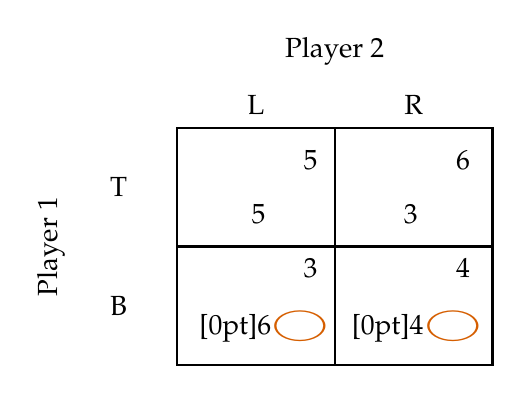
\begin{tikzpicture}
				\matrix[matrix of math nodes,every odd row/.style={align=right},every evenrow/.style={align=left},every node/.style={text width=1.5cm},row sep=0.2cm,column sep=0.2cm,ampersand replacement=\&] (m) {
					5\&6 \\
					5 \&3 \\
					3 \&4 \\
					\Circle{6}\& \Circle{4}\\
				};
				\draw (m.north east) rectangle (m.south west);
				\draw (m.north) -- (m.south);
				\draw (m.east) -- (m.west);
				
				% Player 1
				\coordinate (c) at ($(m.north west)!0.25!(m.south west)$);
				\coordinate (d) at ($(m.north west)!0.75!(m.south west)$);
				\node[left=2pt of c,text width=1cm]  {T};
				\node[left=2pt of d,text width=1cm]  {B};
				
				% Player 2
				\coordinate (a) at ($(m.north west)!0.25!(m.north east)$);
				\coordinate (b) at ($(m.north west)!0.75!(m.north east)$);
				\node[above=5pt of a,anchor=base] {L};
				\node[above=5pt of b,anchor=base] {R};
				
				\node[above=18pt of m.north] (firm b) {Player 2};
				\node[left=1.6cm of m.west,rotate=90,align=center,anchor=center] {Player 1};
				
				%\node[above=5pt of firm b]  {Payoff Matrix};
			\end{tikzpicture}
		\end{column}
	\end{columns}
\end{frame}

\begin{frame}{Simultaneous games: Nash equilibrium}
	\begin{columns}[onlytextwidth, T] 
		\begin{column}{.55\textwidth}
			\begin{wideitemize}
				\item \underline{Step 1}: find the best responses for player 1 and circle them in the payoff matrix.
				\item \underline{Step 2}: find the best responses for player 2 and circle them in the payoff matrix.
			\end{wideitemize}
		\end{column}
		\begin{column}{.45\textwidth}
			%\vspace{30pt}
			\hspace{20pt} 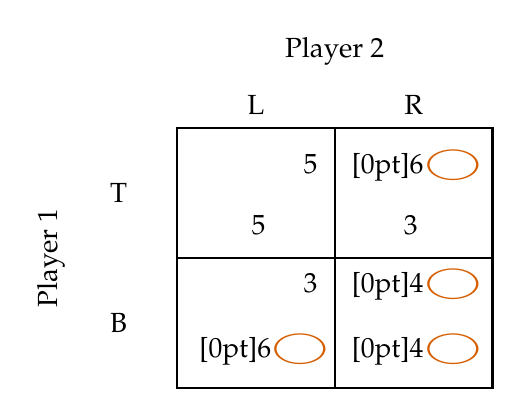
\begin{tikzpicture}
				\matrix[matrix of math nodes,every odd row/.style={align=right},every evenrow/.style={align=left},every node/.style={text width=1.5cm},row sep=0.2cm,column sep=0.2cm,ampersand replacement=\&] (m) {
					5\& \Circle{6} \\
					5\&3 \\
					3 \& \Circle{4} \\
					\Circle{6} \& \Circle{4}\\
				};
				\draw (m.north east) rectangle (m.south west);
				\draw (m.north) -- (m.south);
				\draw (m.east) -- (m.west);
				
				% Player 1
				\coordinate (c) at ($(m.north west)!0.25!(m.south west)$);
				\coordinate (d) at ($(m.north west)!0.75!(m.south west)$);
				\node[left=2pt of c,text width=1cm]  {T};
				\node[left=2pt of d,text width=1cm]  {B};
				
				% Player 2
				\coordinate (a) at ($(m.north west)!0.25!(m.north east)$);
				\coordinate (b) at ($(m.north west)!0.75!(m.north east)$);
				\node[above=5pt of a,anchor=base] {L};
				\node[above=5pt of b,anchor=base] {R};
				
				\node[above=18pt of m.north] (firm b) {Player 2};
				\node[left=1.6cm of m.west,rotate=90,align=center,anchor=center] {Player 1};
				
				%\node[above=5pt of firm b]  {Payoff Matrix};
			\end{tikzpicture}
		\end{column}
	\end{columns}
\end{frame}

\begin{frame}{Simultaneous games: Nash equilibrium}
	\begin{columns}[onlytextwidth, T] 
		\begin{column}{.55\textwidth}
			\begin{wideitemize}
				\item \underline{Step 1}: find the best responses for player 1 and circle them in the payoff matrix.
				\item \underline{Step 2}: find the best responses for player 2 and circle them in the payoff matrix.
				\item \underline{Step 3}: if a box in the payoff matrix has two circles, it is a Nash equilibrium.
				\item So, $(B,R)$ is a Nash equilibrium.
				\begin{wideitemize}
					\item The notation $(B,R)$ means player 1 chooses B, and player 2 chooses R.
				\end{wideitemize}
			\end{wideitemize}
		\end{column}
		\begin{column}{.45\textwidth}
			%\vspace{30pt}
			\hspace{20pt} 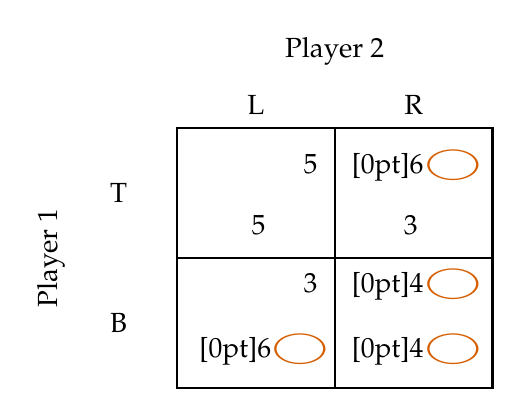
\begin{tikzpicture}
				\matrix[matrix of math nodes,every odd row/.style={align=right},every evenrow/.style={align=left},every node/.style={text width=1.5cm},row sep=0.2cm,column sep=0.2cm,ampersand replacement=\&] (m) {
					5\& \Circle{6} \\
					5\&3 \\
					3 \& \Circle{4} \\
					\Circle{6} \& \Circle{4}\\
				};
				\draw (m.north east) rectangle (m.south west);
				\draw (m.north) -- (m.south);
				\draw (m.east) -- (m.west);
				
				% Player 1
				\coordinate (c) at ($(m.north west)!0.25!(m.south west)$);
				\coordinate (d) at ($(m.north west)!0.75!(m.south west)$);
				\node[left=2pt of c,text width=1cm]  {T};
				\node[left=2pt of d,text width=1cm]  {B};
				
				% Player 2
				\coordinate (a) at ($(m.north west)!0.25!(m.north east)$);
				\coordinate (b) at ($(m.north west)!0.75!(m.north east)$);
				\node[above=5pt of a,anchor=base] {L};
				\node[above=5pt of b,anchor=base] {R};
				
				\node[above=18pt of m.north] (firm b) {Player 2};
				\node[left=1.6cm of m.west,rotate=90,align=center,anchor=center] {Player 1};
				
				%\node[above=5pt of firm b]  {Payoff Matrix};
			\end{tikzpicture}
		\end{column}
	\end{columns}
\end{frame}

\begin{frame}{Simultaneous games: Nash equilibrium}
	\begin{columns}[onlytextwidth, T] 
		\begin{column}{.55\textwidth}
			\begin{wideitemize}
				\item It's possible to have \textit{multiple} Nash equilbria in a game.
				\item When this happens, our simple model makes no predictions about which equilibrium will be observed - all we can say is that the game will end up in \textit{one} of the equilbria.
				\item An example of a game with multiple equilibria is on the right.
				\begin{wideitemize}
					\item I have circled the best responses and the two Nash equilibria are at $(T,L)$ and $(B,R)$
				\end{wideitemize}
			\end{wideitemize}
		\end{column}
		\begin{column}{.45\textwidth}
			%\vspace{30pt}
			\hspace{20pt} 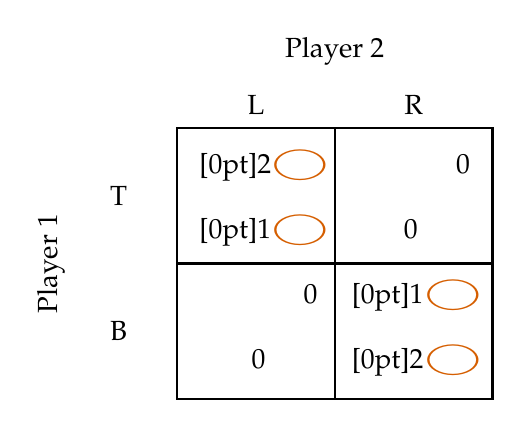
\begin{tikzpicture}
				\matrix[matrix of math nodes,every odd row/.style={align=right},every evenrow/.style={align=left},every node/.style={text width=1.5cm},row sep=0.2cm,column sep=0.2cm,ampersand replacement=\&] (m) {
					\Circle{2} \& 0 \\
					\Circle{1} \& 0 \\
					0 \& \Circle{1} \\
					0 \& \Circle{2} \\
				};
				\draw (m.north east) rectangle (m.south west); 
				\draw (m.north) -- (m.south);
				\draw (m.east) -- (m.west);
				
				% Player 1
				\coordinate (c) at ($(m.north west)!0.25!(m.south west)$);
				\coordinate (d) at ($(m.north west)!0.75!(m.south west)$);
				\node[left=2pt of c,text width=1cm]  {T};
				\node[left=2pt of d,text width=1cm]  {B};
				
				% Player 2
				\coordinate (a) at ($(m.north west)!0.25!(m.north east)$);
				\coordinate (b) at ($(m.north west)!0.75!(m.north east)$);
				\node[above=5pt of a,anchor=base] {L};
				\node[above=5pt of b,anchor=base] {R};
				
				\node[above=18pt of m.north] (firm b) {Player 2};
				\node[left=1.6cm of m.west,rotate=90,align=center,anchor=center] {Player 1};
				
				%\node[above=5pt of firm b]  {Payoff Matrix};
			\end{tikzpicture}
		\end{column}
	\end{columns}
\end{frame}

\begin{frame}{Simultaneous games: prisoner's dilemma}
	\begin{columns}[onlytextwidth, T]
		\begin{column}{.55\textwidth}
			\begin{wideitemize}
				\item Let's look at the first game that we looked at today (rewritten
				on the right). This game is an example of the \textit{prisoner's
				dilemma}.
				\item Let's look at it again with the players and strategies
				relabelled (but with the same payoffs).
				\begin{wideitemize}
					\item The strategies are now to choose prices: a high price `H' or to
				choose a low price `L'.
					\item The interpretation of the payoffs is now profits.
					\item (Note: we could come up with demand, costs, specific prices,
					that generate these profits, but I will ignore this for now.)
				\end{wideitemize}
			\end{wideitemize}
		\end{column}
		\begin{column}{.45\textwidth}
			%\vspace{30pt}
			\hspace{20pt} 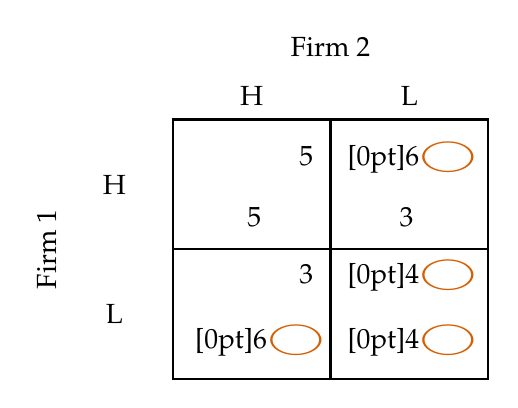
\begin{tikzpicture}
				\matrix[matrix of math nodes,every odd row/.style={align=right},every evenrow/.style={align=left},every node/.style={text width=1.5cm},row sep=0.2cm,column sep=0.2cm,ampersand replacement=\&] (m) {
					5\& \Circle{6} \\
					5\&3 \\
					3 \& \Circle{4} \\
					\Circle{6} \& \Circle{4}\\
				};
				\draw (m.north east) rectangle (m.south west);
				\draw (m.north) -- (m.south);
				\draw (m.east) -- (m.west);

				% Player 1
				\coordinate (c) at ($(m.north west)!0.25!(m.south west)$);
				\coordinate (d) at ($(m.north west)!0.75!(m.south west)$);
				\node[left=2pt of c,text width=1cm]  {H};
				\node[left=2pt of d,text width=1cm]  {L};

				% Player 2
				\coordinate (a) at ($(m.north west)!0.25!(m.north east)$);
				\coordinate (b) at ($(m.north west)!0.75!(m.north east)$);
				\node[above=5pt of a,anchor=base] {H};
				\node[above=5pt of b,anchor=base] {L};

				\node[above=18pt of m.north] (firm b) {Firm 2};
				\node[left=1.6cm of m.west,rotate=90,align=center,anchor=center] {Firm
				1};

				%\node[above=5pt of firm b]  {Payoff Matrix};
			\end{tikzpicture}
		\end{column}
	\end{columns}
\end{frame}

\begin{frame}{Simultaneous games: prisoner's dilemma}
	\begin{columns}[onlytextwidth, T]
		\begin{column}{.55\textwidth}
			\begin{wideitemize}
				\item What can we learn from the prisoner's dilemma?
				\item From the \textit{joint} perspective of both firms, the optimal
				strategies are to choose high prices (H,H). Joint profits will be = 10.
				\item But, from the \textit{individual} perspective of each firm,
				there is an incentive to \textit{deviate} from $(H,H)$.
				\begin{wideitemize}
					\item A firm gets payoff $6>5$ from choosing L when the other firm
					chooses H.
				\end{wideitemize}
				\item Therefore, the game results in a nash equilibrium of (L,L):
				here, joint profits are = 8. This is lower than what is \textit{jointly}
				best
				for the firms!
			\end{wideitemize}
		\end{column}
		\begin{column}{.45\textwidth}
			%\vspace{30pt}
			\hspace{20pt} 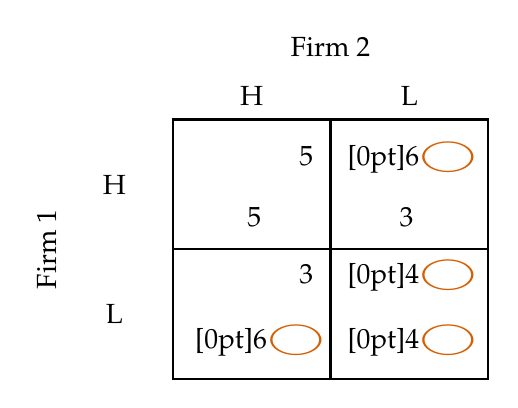
\begin{tikzpicture}
				\matrix[matrix of math nodes,every odd row/.style={align=right},every evenrow/.style={align=left},every node/.style={text width=1.5cm},row sep=0.2cm,column sep=0.2cm,ampersand replacement=\&] (m) {
					5\& \Circle{6} \\
					5\&3 \\
					3 \& \Circle{4} \\
					\Circle{6} \& \Circle{4}\\
				};
				\draw (m.north east) rectangle (m.south west);
				\draw (m.north) -- (m.south);
				\draw (m.east) -- (m.west);

				% Player 1
				\coordinate (c) at ($(m.north west)!0.25!(m.south west)$);
				\coordinate (d) at ($(m.north west)!0.75!(m.south west)$);
				\node[left=2pt of c,text width=1cm]  {H};
				\node[left=2pt of d,text width=1cm]  {L};

				% Player 2
				\coordinate (a) at ($(m.north west)!0.25!(m.north east)$);
				\coordinate (b) at ($(m.north west)!0.75!(m.north east)$);
				\node[above=5pt of a,anchor=base] {H};
				\node[above=5pt of b,anchor=base] {L};

				\node[above=18pt of m.north] (firm b) {Firm 2};
				\node[left=1.6cm of m.west,rotate=90,align=center,anchor=center] {Firm
				1};

				%\node[above=5pt of firm b]  {Payoff Matrix};
			\end{tikzpicture}
		\end{column}
	\end{columns}
\end{frame}

\begin{frame}{Simultaneous games: prisoner's dilemma}
	\begin{wideitemize}
		\item The prisoners dilemma shows the \textit{`conflict between individual incentives and joint incentives'.}
		\item It is an example of why competition might be good for
		consumers, but bad for firms.
			\begin{wideitemize}
		\item If both firm 1 and firm 2 were the same firm (e.g. a monopoly) they would
		choose high prices - this would maximize profits but consumers would have to pay
		high prices.
		\item When the firms are choosing individually (`competing') they undercut each
		other and choose lower prices - this lowers joint profits for firms but consumers
		do better because they pay lower prices.
		\item We will study competition a lot more in the second part of the course.
			\end{wideitemize}
	\end{wideitemize}
\end{frame}

\begin{comment}
\begin{frame}{Simultaneous games: prisoner's dilemma with actual prisoners}
	\begin{columns}[onlytextwidth, T]
	\begin{column}{.55\textwidth}
		\begin{wideitemize}
			\item To see where the name \textit{prisoner's dilemma} comes from, and to practice solving games, let's solve the prisoner's dilemma game with actual prisoners.
			\begin{wideitemize}
				\item Players: Prisoner 1 and Prisoner 2
				\item Strategies: Confess (`C') or Do Not Confess ('DNC')
				\item Payoffs: (Negative) years in jail (so higher is better)
			\end{wideitemize}
			\item Nash Equilbrium: (C,C) both players confess and each get 8 years jail. But: if neither player were to confess (DNC, DNC) they would only get 1 year each in jail.
		\end{wideitemize}
	\end{column}
	\begin{column}{.45\textwidth}
		%\vspace{30pt}
		\hspace{20pt} 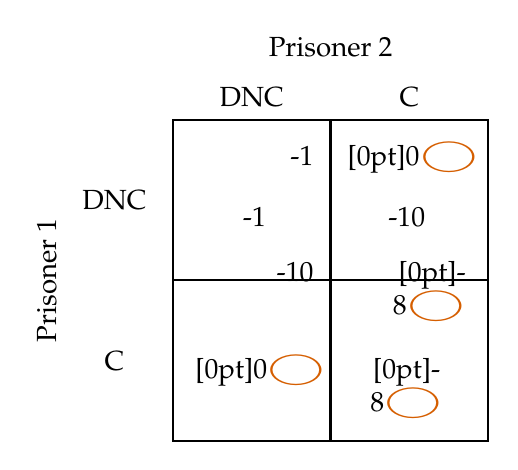
\begin{tikzpicture}
			\matrix[matrix of math nodes,every odd row/.style={align=right},every evenrow/.style={align=left},every node/.style={text width=1.5cm},row sep=0.2cm,column sep=0.2cm,ampersand replacement=\&] (m) {
				-1\& \Circle{0} \\
				-1\&-10 \\
				-10 \& \Circle{-8} \\
				\Circle{0} \& \Circle{-8}\\
			};
			\draw (m.north east) rectangle (m.south west);
			\draw (m.north) -- (m.south);
			\draw (m.east) -- (m.west);
			
			% Player 1
			\coordinate (c) at ($(m.north west)!0.25!(m.south west)$);
			\coordinate (d) at ($(m.north west)!0.75!(m.south west)$);
			\node[left=2pt of c,text width=1cm]  {DNC};
			\node[left=2pt of d,text width=1cm]  {C};
			
			% Player 2
			\coordinate (a) at ($(m.north west)!0.25!(m.north east)$);
			\coordinate (b) at ($(m.north west)!0.75!(m.north east)$);
			\node[above=5pt of a,anchor=base] {DNC};
			\node[above=5pt of b,anchor=base] {C};
			
			\node[above=18pt of m.north] (firm b) {Prisoner 2};
			\node[left=1.6cm of m.west,rotate=90,align=center,anchor=center] {Prisoner
				1};
			
			%\node[above=5pt of firm b]  {Payoff Matrix};
		\end{tikzpicture}
	\end{column}
\end{columns}
\end{frame}
\end{comment}

\begin{frame}{Simultaneous games: finding Nash Equilibria in complicated games, p164-p165}
		\begin{figure}
			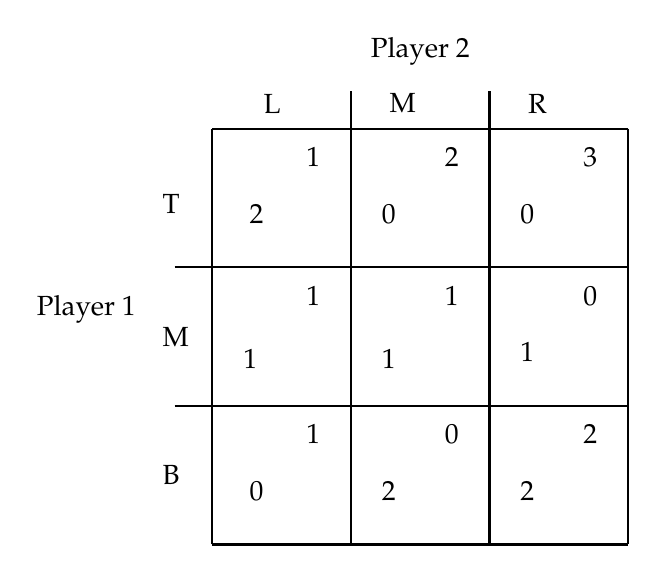
\begin{tikzpicture}[scale=1.6]
				\draw[ thick ] (0,0) -- (3.3,0);
				\draw[ thick ] (0,0) -- (0,3.3);
				\draw[ thick ] (3.3,3.3) -- (3.3,0);
				\draw[ thick ] (3.3,3.3) -- (0,3.3);	
				\draw[ thick ] (-0.3,1.1) -- (3.3,1.1);
				\draw[ thick ] (-0.3,2.2) -- (3.3,2.2);
				\draw[ thick ] (1.1,0) -- (1.1,3.6);
				\draw[ thick ] (2.2,0) -- (2.2,3.6);
				
				\coordinate[label= right:T] (p1) at (-0.5,2.7);
				\coordinate[label= right:M] (p1) at (-0.5,1.65);
				\coordinate[label= right:B] (p1) at (-0.5,0.55);
				\coordinate[label= right:L] (p1) at (0.3,3.5);
				\coordinate[label= right:M] (p1) at (1.3,3.5);
				\coordinate[label= right:R] (p1) at (2.4,3.5);
				
				\coordinate[label= above:Player 2] (p1) at (1.65,3.7);
				\coordinate[label= above:Player 1] (p1) at (-1.0,1.65);
				
				%mid-left
				\fill[black] (0.3,1.4) node {$1$};
				\fill[black] (0.8,1.9) node {$1$};
				
				%mid-middle
				\fill[black] (1.4, 1.4) node {$1$};
				\fill[black] (1.9,1.9) node {$1$};
				
				%bot-left
				\fill[black] (0.35, 0.35) node {$0$};
				\fill[black] (0.8, 0.8) node {$1$};
				
				%bot-mid
				\fill[black] (1.4, 0.35) node {$2$};
				\fill[black] (1.9, 0.8) node {$0$};
				
				%bot-right
				\fill[black] (2.5, 0.35) node {$2$};
				\fill[black] (3.0, 0.8) node {$2$};
				
				%mid-right
				\fill[black] (2.5, 1.45) node {$1$};
				\fill[black] (3.0, 1.9) node {$0$};
				
				%top-right
				\fill[black] (2.5, 2.55) node {$0$};
				\fill[black] (3.0, 3.0) node {$3$};
				
				%top-middle
				\fill[black] (1.4, 2.55) node {$0$};
				\fill[black] (1.9, 3.0) node {$2$};
				
				%top-left
				\fill[black] (0.35, 2.55) node {$2$};
				\fill[black] (0.8, 3.0) node {$1$};
			\end{tikzpicture}
		\end{figure}
\end{frame}

\begin{frame}{Simultaneous games: finding Nash Equilibria in complicated games, p164-p165}
		\begin{wideitemize}
		\item Nash equilibrium at (B,R).
	\end{wideitemize}
	\begin{figure}
		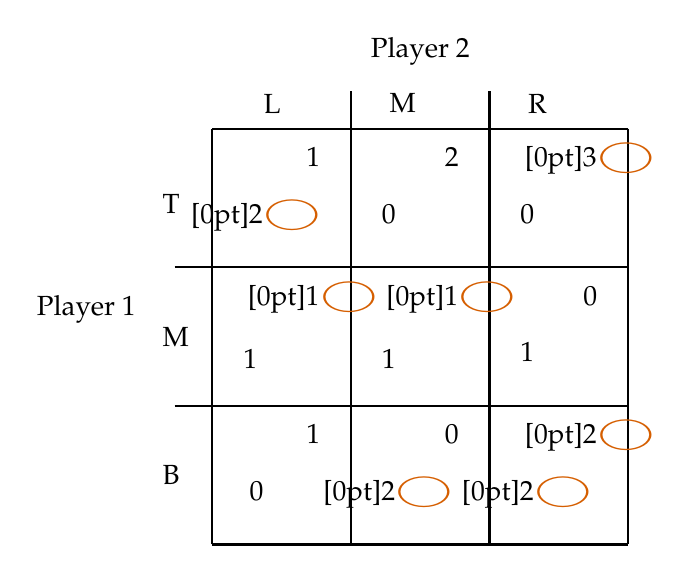
\begin{tikzpicture}[scale=1.60]
			\draw[ thick ] (0,0) -- (3.3,0);
			\draw[ thick ] (0,0) -- (0,3.3);
			\draw[ thick ] (3.3,3.3) -- (3.3,0);
			\draw[ thick ] (3.3,3.3) -- (0,3.3);	
			\draw[ thick ] (-0.3,1.1) -- (3.3,1.1);
			\draw[ thick ] (-0.3,2.2) -- (3.3,2.2);
			\draw[ thick ] (1.1,0) -- (1.1,3.6);
			\draw[ thick ] (2.2,0) -- (2.2,3.6);
			
			\coordinate[label= right:T] (p1) at (-0.5,2.7);
			\coordinate[label= right:M] (p1) at (-0.5,1.65);
			\coordinate[label= right:B] (p1) at (-0.5,0.55);
			\coordinate[label= right:L] (p1) at (0.3,3.5);
			\coordinate[label= right:M] (p1) at (1.3,3.5);
			\coordinate[label= right:R] (p1) at (2.4,3.5);
			
			\coordinate[label= above:Player 2] (p1) at (1.65,3.7);
			\coordinate[label= above:Player 1] (p1) at (-1.0,1.65);
			
			%mid-left
			\fill[black] (0.3,1.4) node {$1$};
			\fill[black] (0.8,1.9) node {\Circle{$1$}};
			
			%mid-middle
			\fill[black] (1.4, 1.4) node {$1$};
			\fill[black] (1.9,1.9) node {\Circle{$1$}};
			
			%bot-left
			\fill[black] (0.35, 0.35) node {$0$};
			\fill[black] (0.8, 0.8) node {$1$};
			
			%bot-mid
			\fill[black] (1.4, 0.35) node {\Circle{$2$}};
			\fill[black] (1.9, 0.8) node {$0$};
			
			%bot-right
			\fill[black] (2.5, 0.35) node {\Circle{$2$}};
			\fill[black] (3.0, 0.8) node {\Circle{$2$}};
			
			%mid-right
			\fill[black] (2.5, 1.45) node {$1$};
			\fill[black] (3.0, 1.9) node {$0$};
			
			%top-right
			\fill[black] (2.5, 2.55) node {$0$};
			\fill[black] (3.0, 3.0) node {\Circle{$3$}};
			
			%top-middle
			\fill[black] (1.4, 2.55) node {$0$};
			\fill[black] (1.9, 3.0) node {$2$};
			
			%top-left
			\fill[black] (0.35, 2.55) node {\Circle{$2$}};
			\fill[black] (0.8, 3.0) node {$1$};
		\end{tikzpicture}
	\end{figure}
\end{frame}

\begin{frame}{Plan}
	\begin{wideenumerate}
		\item Simultaneous games: setup and Nash equilibrium
		\item \textbf{Simultaneous games: dominant and dominated strategies}
	\end{wideenumerate}
\end{frame}


\begin{frame}{Dominant and dominated strategies}
	\begin{wideitemize}
		\item We give names to certain types of strategies.
		\item One is a \textbf{dominant strategy}:
		\begin{wideitemize}
			\item \textit{A dominant strategy yields a player the highest payoff regardless of the other players choices.}
		\end{wideitemize}
		\item One is a \textbf{dominated strategy}:
		\begin{wideitemize}
			\item \textit{A dominanted strategy yields a player a payoff which is lower than that of a different strategy, regardless of what the other players do.}
		\end{wideitemize}
		\item Note: for many games, there are no dominant or dominated strategies.
	\end{wideitemize}
\end{frame}

\begin{frame}{Dominant and dominated strategies: prisoner's dilemma}
	\begin{columns}[onlytextwidth, T]
		\begin{column}{.5\textwidth}
			%\vspace{30pt}
			\hspace{20pt} 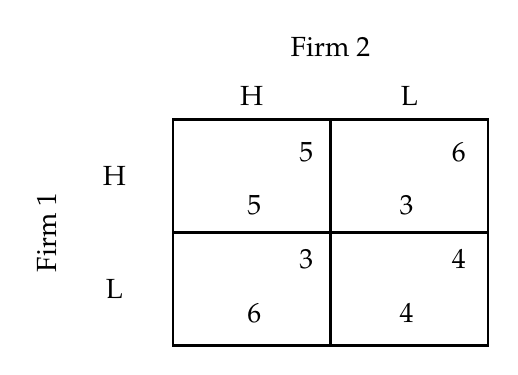
\begin{tikzpicture}
				\matrix[matrix of math nodes,every odd row/.style={align=right},every evenrow/.style={align=left},every node/.style={text width=1.5cm},row sep=0.2cm,column sep=0.2cm,ampersand replacement=\&] (m) {
					5\& 6 \\
					5\&3 \\
					3 \& 4 \\
					6 \& 4 \\
				};
				\draw (m.north east) rectangle (m.south west);
				\draw (m.north) -- (m.south);
				\draw (m.east) -- (m.west);
				
				% Player 1
				\coordinate (c) at ($(m.north west)!0.25!(m.south west)$);
				\coordinate (d) at ($(m.north west)!0.75!(m.south west)$);
				\node[left=2pt of c,text width=1cm]  {H};
				\node[left=2pt of d,text width=1cm]  {L};
				
				% Player 2
				\coordinate (a) at ($(m.north west)!0.25!(m.north east)$);
				\coordinate (b) at ($(m.north west)!0.75!(m.north east)$);
				\node[above=5pt of a,anchor=base] {H};
				\node[above=5pt of b,anchor=base] {L};
				
				\node[above=18pt of m.north] (firm b) {Firm 2};
				\node[left=1.6cm of m.west,rotate=90,align=center,anchor=center] {Firm
					1};
				
				%\node[above=5pt of firm b]  {Payoff Matrix};
			\end{tikzpicture}
		\end{column}
		\begin{column}{.5\textwidth}
			\begin{wideitemize}
				\item As an example of dominant and dominated strategies, let's revisit the prisoner's dilemma.
				\item Are there dominant and dominated strategies in this game? 
				\pause
				\item Yes! 
				\item For Firm 1: L is the dominant strategy, H is the dominated strategy
				\item For Firm 2: L is the dominant strategy, H is the dominated strategy
			\end{wideitemize}
		\end{column}
	\end{columns}
\end{frame}

\begin{frame}{Dominated strategies: example}
	\begin{columns}[onlytextwidth, T]
		\begin{column}{.5\textwidth}
		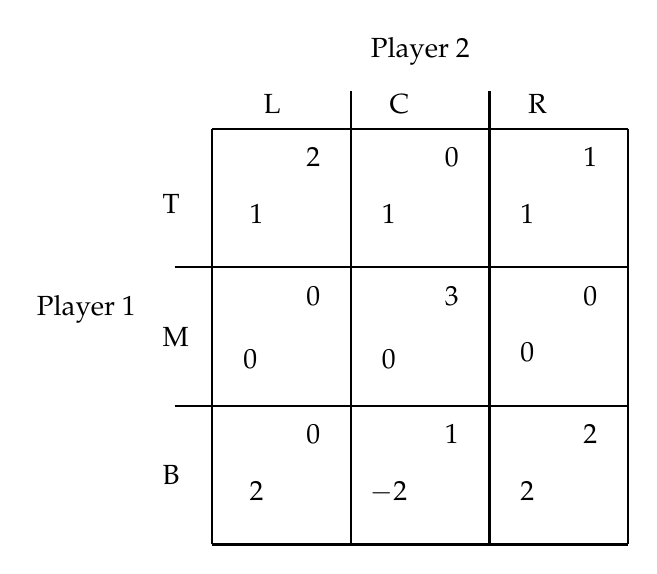
\begin{tikzpicture}[scale=1.6]
	\draw[ thick ] (0,0) -- (3.3,0);
	\draw[ thick ] (0,0) -- (0,3.3);
	\draw[ thick ] (3.3,3.3) -- (3.3,0);
	\draw[ thick ] (3.3,3.3) -- (0,3.3);	
	\draw[ thick ] (-0.3,1.1) -- (3.3,1.1);
	\draw[ thick ] (-0.3,2.2) -- (3.3,2.2);
	\draw[ thick ] (1.1,0) -- (1.1,3.6);
	\draw[ thick ] (2.2,0) -- (2.2,3.6);
	
	\coordinate[label= right:T] (p1) at (-0.5,2.7);
	\coordinate[label= right:M] (p1) at (-0.5,1.65);
	\coordinate[label= right:B] (p1) at (-0.5,0.55);
	\coordinate[label= right:L] (p1) at (0.3,3.5);
	\coordinate[label= right:C] (p1) at (1.3,3.5);
	\coordinate[label= right:R] (p1) at (2.4,3.5);
	
	\coordinate[label= above:Player 2] (p1) at (1.65,3.7);
	\coordinate[label= above:Player 1] (p1) at (-1.0,1.65);
	
	%mid-left
	\fill[black] (0.3,1.4) node {$0$};
	\fill[black] (0.8,1.9) node {$0$};
	
	%mid-middle
	\fill[black] (1.4, 1.4) node {$0$};
	\fill[black] (1.9,1.9) node {$3$};
	
	%bot-left
	\fill[black] (0.35, 0.35) node {$2$};
	\fill[black] (0.8, 0.8) node {$0$};
	
	%bot-mid
	\fill[black] (1.4, 0.35) node {$-2$};
	\fill[black] (1.9, 0.8) node {$1$};
	
	%bot-right
	\fill[black] (2.5, 0.35) node {$2$};
	\fill[black] (3.0, 0.8) node {$2$};
	
	%mid-right
	\fill[black] (2.5, 1.45) node {$0$};
	\fill[black] (3.0, 1.9) node {$0$};
	
	%top-right
	\fill[black] (2.5, 2.55) node {$1$};
	\fill[black] (3.0, 3.0) node {$1$};
	
	%top-middle
	\fill[black] (1.4, 2.55) node {$1$};
	\fill[black] (1.9, 3.0) node {$0$};
	
	%top-left
	\fill[black] (0.35, 2.55) node {$1$};
	\fill[black] (0.8, 3.0) node {$2$};
\end{tikzpicture}
		\end{column}
		\begin{column}{.5\textwidth}
			\begin{wideitemize}
				\item Let's solve the game from before using \textit{iterated deletion of dominated strategies}.
				\begin{wideitemize}
					\item Essentially, keep deleting dominated strategies until we reach a Nash equilibrium.
									\pause
					\item For player 1, M is a dominated action. Eliminate it (cross it out) of the game.
					\item Given the above, C is dominated for player 2. Eliminate it from the game.
					\item Given the above, T is dominated for player 1. Eliminate it.
					\item Finally, given the above, L is a dominated strategy for player 2. Eliminate it.
					\item What is left: Nash equilbrium at (B,R).
				\end{wideitemize}
			\end{wideitemize}
		\end{column}
	\end{columns}
\end{frame}

\begin{frame}{Summary of key points*}
	%\vspace{-20pt}
	\begin{wideitemize}
		\item Know how to identify the components of a simultaneous game: players, strategies, payoffs
		\item Know how to compute best responses
		\item Compute Nash equilibrium from best responses, and understand the the predictions of a Nash equilibrium rely on assumptions about whether the players are choosing \textit{rationally}
		\item Understand the prisoner's dilemma illustrates the `conflict between individual incentives and joint incentives'.
		\item Know what a `dominant' and `dominated' strategy are.
		\item Solve games using iterated deletion of dominated strategies.
	\end{wideitemize}
	\vspace{20pt}
	*To clarify, all the material in the slides, problem sets, etc is assessable unless stated otherwise, but I hope this summary might be a useful place to start when studying the material.
\end{frame}

%\begin{frame}{The discrete Bertrand game (p186)}
	%\begin{wideitemize}
		%\item \textbf{Question}: Two firms set prices simultaneously. Consumers buy from the firm with the lowest price and split their demand equally across the two firms if prices are equal. Market demand is $q=10-p$, $MC=2$. Sellers can only set the following prices: $3,4,5$.
		%\item 1. Write down the normal form game.
		%\item 2. Solve for the equilibrium of the game.
	%\end{wideitemize}
%\end{frame}

\end{document}
